% EvangelosPHYS7123.tex

% add editing date at the top  whenever any file.tex is modified
% ES 							Feb 3:
% http://publish.aps.org/esubs/revtextips.html

% this style for submission, web version:
%\documentclass[pre,twocolumn,groupedaddress,showpacs,showkeys]{revtex4}

% this style while editing:
\documentclass[pre,preprint,groupedaddress,showpacs,showkeys]{revtex4}

\usepackage{hyperref}
%\usepackage[active]{srcltx}



\input defs	  		% all definitions in defs.tex
				\begin{document}
				\title{
Penalizing loops that deviate from the True Path.
				}\author{
Evangelos Siminos				}\email{gtg083n@mail.gatech.edu}
\affiliation{
		School of Physics\\
		Georgia Institute of Technology, Atlanta, GA 30332-0430, U.S.A}
				\date{April 5, 2005} % or edit manually:
				%\date{November 11,:}

				\begin{abstract}
 A variational method for periodic orbit searches in a general flow is developed.
 The method is based on penalizing the misorientation of the tangent vector of a guess-loop to
 the velocity field of the given flow. The loop is continuously evolved into a periodic orbit 
 by a fictitious time flow. The main goal of the project is the definition of a natural and 
 advantageous (i.e. informed of the flow) metric in the space of loops.

\end{abstract}
\pacs{95.10.Fh, 02.70.Bf, 47.52.+j, 05.45.+a}
\keywords{
periodic orbits, 
chaos, turbulence
	} 
					\maketitle

\noindent
{\bf Georgia Tech PHYS 7224:}\\
\underline{\bf CHAOS, AND WHAT TO DO ABOUT IT }\\
{\bf course project, spring semester 2005}

\section{Introduction}

 The goal of this project is to improve the variational method
 for finding periodic orbits introduced in \refrefs{lanVar1,CvitLanCrete02}.
 The method evolves an initial guess in the form of a closed loop $L$
 towards a periodic orbit $p$ of a given flow $f^t(x)$ defined by:
 \beq
    \frac{dx}{dt}=v(x),\; x \in \mathbb{R}^{d+1}\, .
    \label{eq:flow}
 \eeq
% This is achieved by minimizing the misorientation of the 
%unit tangent vector $\hat{t}(x)$ of the loop to the unit vector $\hat{v}(x)$ parallel to %the velocity field \refeq{eq:flow}. In other words minimizing the cost functional    
% \beq
%    \overline{F}^2=\frac{1}{L} \oint\left(\hat{t}-\hat{v} \right)^2 \, dl \,,
%    \label{eq:simplefunctional}
% \eeq
% where the integration is performed along the loop.

% The improvement that will be pursued here is to replace the
% simple Euclidean metric $\delta_{ij}$ that is used in \refeq{eq:simplefunctional}
% with a metric $g_{ij}$ that would carry information about the flow, \ie \ 
% minimize the functional
% \beq
%    \overline{F}^2=\frac{1}{L}\oint\left(\hat{t}-\hat{v} \right)_i\, 			%			g_{ij}\,\left(\hat{t}-\hat{v}\right)_j \, dl \,.
%    \label{eq:functional}
% \eeq
 
Given a loop parameterized by a parameter $s$, this is achieved by minimizing the misorientation of the tangent vector $\tilde{v}(x)=dx/ds$ of the loop to the velocity vector \refeq{eq:flow}. Locally,
the loop deviates from the true flow by the misalignment of the loop tangent vector
\beq
	F(x)=v(x)-\lambda(x)\tilde{v}(x)\,,\ x=x(s)\in L\,.	
\eeq
 $\lambda(x)$ is an auxiliary undetermined function which compensates for the fact that not only the direction, 
 but also the magnitudes of the two fields need to be equal on a periodic orbit. A cost functional    
 \beq
    F^2=\frac{1}{S} \oint_L\left(v(x)-\lambda(x)\, \tilde{v}(x) \right)^2 \, ds \,,
    \label{eq:simplefunctional}
 \eeq
 is an indication of the deviation of the of the guess loop $L$ from a periodic orbit of the 
 flow \refeq{eq:flow}. Here $S$ is a normalization factor.

 The improvement that will be pursued here is to replace the
 simple Euclidean metric $\delta_{ij}$ that is used in \refeq{eq:simplefunctional}
 with a metric $g_{ij}(x)$ that would carry information about the flow, \ie \ 
 minimize the functional
 \beq
    F^2=\frac{1}{S}\oint\left(v-\lambda \tilde{v} \right)_i\, 					
    			g_{ij}\,\left(v-\lambda \tilde{v} \right)_j \, ds \,.
    \label{eq:functional}
 \eeq
 
 
 
\section{Variational searches for periodic orbits}
\label{sec:der}

 In this project any smooth, closed curve in our $d+1-$dimensional space is referred
 to as a loop $L$. In general a loop is not a solution 
 of \refeq{eq:flow}, in contrast to a periodic orbit, which satisfies
 the periodic orbit condition $f^T(x)=x$, where $T$ the period. The
 loop tangent vector $\tilde{v}$ is in general not parallel to 
 $\hat{v}$. Thus, if we could continously deform the loop in such
 a way that its tangent becomes parallel to the velocity field everywere we would end up
 with a periodic orbit. In \refref{CvitLanCrete02} it is shown that this
 corresponds to minimizing \refeq{eq:simplefunctional} and that one can write down
 a partial differential equation (PDE) for the evolution of the loop towards 
 a periodic orbit. As the form of the equation depends on the parameterization
 of the loop and the choice of metric, such a PDE will only be presented here
 for our specific choices, \cf\ \refsect{sec:PDE-eucl}. Numerically solving
 this PDE provides the periodic orbit of the system ``closest'' to the initial loop.
 Distance in the space of loops is hard to define. In practice the method converges to a loop with 
 topology ``similar'' to the initial guess. 
 
 The method is conceptually more complicated, harder to program and generally
 slower than Newton or multiple-shooting methods for the search of periodic
 orbits. On the other hand it has an advantage when one tries to find long
 or extremely unstable periodic orbits, or when one deals with hard-to-visualize \
 high-dimensional systems. For multiple-shooting to converge one needs a
 large number of Poincar\'e sections in order to control local instability.
 Thus one needs a great deal of information about the qualitative dynamics
 of the flow to make a clever choice of those sections. In high-dimensional flows
 this information is usually not available and multiple shooting methods can easily fail
 to find the longer cycles. In the variational method described
 here Poincar\'e sections play no role and guesses with roughly the
 correct topology can lead to long cycles. In practice one constructs guess-loops by patching
 together pieces of trajectories to form a discontinuous loop, transforms in Fourier space and
 drops the high-frequency components to get a closed curve, \cf\ \refref{lanVar1}  
 
 The extension of the method that will be attempted here is to use a metric
 that penalizes variations from a true periodic orbit in the unstable eigendirections
 of the flow more than it does in the stable ones. The hope is that in a high-dimensional
 flow in which only a few of the these eigendirections are significant, one can concentrate on them,
 effectively reducing the dimensionality of the problem and the computational load.  
 
\section{Candidates for the role of Metric}

 \subsection{A Jacobian Matrix for a Loop}
 
  The Jacobian matrix $\mathbf{J}^t(x_o)$ describes the deformation of the neighborhood 
  of a point $x_o$ under a flow $f^t$, in the linear approximation,
  \beq
  	\mathbf{J}^t_{ij}(x_o)=\left. \fp{f^t_i(x_o)_i}{x_{o_j} }\right|_{x=x_o} \, .
	\label{eq:def:J}
  \eeq
  Using \refeq{eq:def:J} one can show (e.g. \cf\ \refref{DasBuch}, Chapter 4) that the Jacobian can be computed by means of the time-ordered product 
  \bea
  	\mathbf{J}^t(x_o) & = & \mathbf{T} e^{\int_0^t d\tau  \mathbf{A}\left(f^{\tau}(x_o)\right)} 		\continue
			& = &  \lim_{m\rightarrow \infty} \prod_{n=m}^1
			  	e^{ \Delta t \, \mathbf{A}\left(f^{n \Delta t}(x_o)\right) }\,, 
	\label{eq:def:Jacobian}
  \eea
  where $\Delta t= t/m$ and $\mathbf{A}$ the matrix of variations defined by
  \beq
  	A_{ij}(x)=\frac{\partial v_i}{\partial x_j}\,.
  \eeq
  Along a periodic orbit
    \beq
  	\mathbf{J}_p\equiv \mathbf{J}^{T_p}(x_o) = \mathbf{T} e^{\oint d\tau  \mathbf{A}\left(f^{\tau}(x_o)\right)} \,.
	\label{eq:Jp}
  \eeq
  $\mathbf{J}_p$ describes the local deformation of the neighborhood of the periodic
   orbit under the flow. Its eigenvalues are independent of the initial point $x_o$ on the periodic
   orbit, and provide the local measure of instability of the system.
   
   Thus we would like to use $\mathbf{J}$ as our metric tensor. Yet,
   a loop is not a solution of the equations of the flow
   and we cannot calculate the Jacobian along it. Inspired by the time-ordered 
   product \refeq{eq:def:Jacobian}, we \emph{define} the Jacobian along any path as
   \bea
  	\Js^s(x_o) & \equiv & \mathbf{T} e^{\int ds\,  \dtds\, \mathbf{A}\left(x(s))\right)} 		\continue
			& \equiv &  \lim_{m\rightarrow \infty} \prod_{n=m}^1
			  	e^{ \Delta s \,\dtds\, \mathbf{A}\left(x(n\, \Delta s)\right) }\,, 
	\label{eq:def:sJacobian}
  \eea 
   where $s\in[s_i,s_f]$ parameterizes the path, $\Delta s = (s_f-s_i)/m$ and $\mathbf{T}$ now
   reminds us that the integration is ordered with respect to $s$. We will denote $\Js(x_o)$ evaluated 
   around a closed loop, starting at point $x_o(s)$ as $\JL(x_o)$.
   
   Obviously, $\Js^s(x_o)$ is a solution of the differential equation
   \beq
   	\fd{\Js^s(x_o)}{s}=\dtds\,\mathbf{A}(x(s))\,\Js^s(x_o).
	\label{eq:difJ}
   \eeq 
   


 \subsection{Properties of $\JL$}
 
  We now prove that $\JL$ shares with $\Jp$ the property that its eigenvalues do not 
  depend on the initial point on the loop. Definition \refeq{eq:def:sJacobian} establishes 
  the group property
  \beq
  	\Js^{s+s'}(x_o)
		=\Js^{s'}(x(s))\Js^{s}(x_o)\,.
	\label{eq:Jgroup}
  \eeq
  
  Next we consider the eigenvalue-eigenvector equation for $\JL$
  \beq
  	\JL(x) e_i(x)=\Lambda_{L,i} e_i(x)\,,
	\label{eq:Jeig}
  \eeq
  with $\JL$ evaluated at a specific point $x(s)$. At a different point on the loop $x'(s')$ we have
  the Jacobian $\JL(x')$. Let $S_L$ be the ``period'' of the loop in $s$ and $\Delta s=s'-s$. Using  \refeq{eq:Jgroup} we can write
  \beq
  	\Js^{S_L+\Delta s}(x)  = \Js^{S_L}(x')\Js^{\Delta s}(x) =\JL(x')\Js^{\Delta s}(x)\,,
  \eeq
  and also
  \beq
  	\Js^{\Delta s+S_L}(x)  = \Js^{\Delta s}(x)\Js^{S_L}(x) = \Js^{\Delta s}(x)\JL(x)\,.
  \eeq
  Thus
  \beq
 	\Js^{\Delta s}(x)\JL(x)=\JL(x')\Js^{\Delta s}(x)\,.
	\label{eq:StrangeCommutation}
  \eeq 
  Multiply \refeq{eq:Jeig} with $\Js^{\Delta s}(x)$ and use \refeq{eq:StrangeCommutation} to get
  \beq
  	\JL(x')\Js^{\Delta s}(x)e_i(x)=\Lambda_{L,i} \Js^{\Delta s}(x)e_i(x)\,.
  \eeq   
  But this is the eigenvalue-eigenvector equation for $\JL(x')$. Thus $\JL(x')$ has the same eigenvalues
  $\Lambda_{L,i}$ as $\JL(x)$, but corresponding eigenvectors
  \beq
  	e_i(x')\equiv \Js^{\Delta s}(x)e_i(x)\,,
  \eeq 
  \ie, the eigenvectors are transported by the Jacobian matrix $\Js^{\Delta s}(x)$. The case of the Jacobian
  for a periodic orbit $\Jp(x)$ is a special case of this result. The crucial part for the proof was the
  group property \refeq{eq:Jgroup} and not the specific definition of $\Js$ or the fact that it was computed
  along a loop and not a periodic orbit. 
  
  We would also like to prove that the eigenvalues of $\JL$ are invariant under a change of
  variables, $y=h(x)$. For notational simplicity we temporarilly drop the tilde in $\Js$.
  Let $\mathbf{\hat{J}}^s(y_o)$ denote the Jacobian for the loop in the new variables, with $y_o=h(x_o)$.
  Then, according to the definition of the Jacobian on a loop
  \beq
   	\frac{d\mathbf{\hat{J}}^s}{ds}=\hdtds\mathbf{\hat{A}}\mathbf{\hat{J}}^s\,,
	\label{eq:difhatJ}
  \eeq
  where $\hat{A}_{ij}= \frac{\partial u_i}{\partial y_j}$ the matrix of variations in the new
  coordinates and
  \bea
  	u_i & = & \fd{y_i}{t} \continue
	 	& = & \fp{h_i}{x_j} v_j \,.
  \eea
  From now on we adopt the convention of summing over repeated indices.
  For notational compactness we define the matrix
  \beq
  	H_{ij}=\fp{h_i}{x_j}\,.
  \eeq 
  Then, for the matrix elements of $\mathbf{\hat{A}}$ we have
  \bea
 	\hat{A}_{ij} & = & \frac{\partial u_i}{\partial y_j} \continue
		& = & \frac{\partial u_i}{\partial x_k}\frac{\partial x_k}{\partial y_j} \continue
		& = & \frac{\partial}{\partial x_k} \left(H_{im} v_m \right)
				\frac{\partial x_k}{\partial y_j} \continue
		& = &  \left(\fp{H_{im}}{x_k}v_m + H_{im} A_{mk} \right)H^{-1}_{kj}\,,
	\label{eq:uv}			
  \eea
  where $H^{-1}_{ij}=\fsp{h^{-1}_i}{y_j}$. 
  
  To relate the eigenvalues of $\mathbf{J}$ and $\mathbf{\hat{J}}$ we form the matrix
  \beq
  	\mathbf{N}^s \equiv \mathbf{\hat{J}}^s(y_o)-\mathbf{H}(x(s)) \mathbf{J}^s(x_o) \mathbf{H}^{-1}(x_o)\,,
	\label{eq:def:N}
  \eeq
  Differentiating with respect to $s$, 
  \beq
  	\fd{N_{ij}^s}{s}  =  \fd{\hat{J}_{ij}^s}{s}-\fd{H_{im}}{s}J^s_{mk}H^{-1}_{kj}
						-H_{im}\fd{J^s_{mk}}{s}H^{-1}_{kj} \,,
  \eeq
  or, using \refeq{eq:difJ} and \refeq{eq:difhatJ},
  \beq
	\fd{N_{ij}^s}{s}  = \hdtds\hat{A}_{im} \hat{J}^s_{mj}-\fp{H_{im}}{x_n}\fd{x_n}{s}J_{mk}H^{-1}_{kj}
						-H_{im} \dtds A_{mn}J^s_{nk}H^{-1}_{kj} \,.
  \eeq
  With the use of \refeq{eq:uv} and renaming of the dummy indices $n\leftrightarrow m$ in the last term, this reads
  \beq	
	\fd{N_{ij}^s}{s} = \hdtds \left(\fp{H_{in}}{x_k}v_n + H_{in} A_{nk} \right)
				H^{-1}_{km}(x(s)) \hat{J}^s_{mj} 
				-\left(\fp{H_{im}}{x_n}\fd{x_n}{s}
						+\dtds H_{in} A_{nm}\right)J^s_{mk}H^{-1}_{kj}(x_o) \,.
  \eeq
  Inserting the identity matrix $\mathbf{1} = \mathbf{H}^{-1}(x(s))\mathbf{H}(x(s))$ in the second term, noting that
  \beq
  	\fp{H_{in}}{x_k}=\fps{h_i}{x_k}{x_n}=\fp{H_{ik}}{x_n}\,,
  \eeq
  and using the fact that $\dtds=\hdtds=\fd{t}{s}$ we get
  \bea
	\fd{N_{ij}^s}{s} & = &  \left(\fp{H_{ik}}{x_n} \fd{x_n}{s} + \fd{t}{s} H_{in} A_{nk} \right)
				H^{-1}_{km}(x(s)) \hat{J}^s_{mj} 
				-\left(\fp{H_{im}}{x_n}\fd{x_n}{s}
						+\fd{t}{s}H_{in}A_{nm}\right)H^{-1}_{mq}H_{ql}J^s_{lk}H^{-1}_{kj}(x_o) \continue
			& = & \left(\fp{H_{ik}}{x_n} \fd{x_n}{s} + \fd{t}{s} H_{in} A_{nk} \right) H^{-1}_{km} N_{mj} \,,
	\label{eq:dNds}
  \eea
  where we used \refeq{eq:def:N} in the last step.  The initial condition is found from \refeq{eq:def:N} 
  to be $\mathbf{N}^0=0$ and thus the solution will be $\mathbf{N}^s \equiv 0$ for every $s$. Thus
 \beq
 	\mathbf{\hat{J}}^s(y_o)=\mathbf{H}(x(s))\mathbf{J}^s\mathbf{H}^{-1}(x_o)\,.
 \eeq  
 On a closed loop we have $x(S)=x_o$ and thus
 \beq
 	\mathbf{\hat{J}}_L(y_o)=\mathbf{H}(x_o)\mathbf{J}_L\mathbf{H}^{-1}(x_o)\,,
 \eeq
 which means that $\mathbf{\hat{J}}_L$ and $\mathbf{J}_L$ are related by a similarity transformation and therefore
 share the same eigenvalues. 
  
  

   
    
\subsection{The variational method}

 We will try to motivate our variational method in terms of the path integral formulation of a random walk, \cf\ \refref{Risken}.
 We consider a discretized loop consisting of $N$ point. At each point $x_i$ we form the difference $x_{i+1}-f^{\Delta t_i}(x)$, where $x_i+1$
 the next point on the loop and $f^{\Delta t_i}(x_i)$  the point at which the flow would transport $x_i$ at time $\Delta t_i$. 
 On a periodic orbit the cost function 
 \beq
 	F^2  =  \sum_{i=0}^N \frac{1}{\Delta t_i}\left(x_{i+1}-f^{\Delta t_i}(x_i) \right)^2
 \eeq
 is obviously equal to zero, and since it is a positive definite quantity this value would be a minimum. The factor of $\Delta t_i$ has been used
 so that the cost function has the dimensions of a diffusion constant in agreement with the stochastic integral formulation. We rewrite this quantity
 as
 \bea
	F^2	& = & \sum_{i=0}^N \frac{1}{\Delta t_i}\left(x_{i+1}-x_i-f^{\Delta t_i}(x_i)-x_i \right)^2 \continue
		& = & \sum_{i=0}^N \Delta t_i \left(\frac{x_{i+1}-x_i}{\Delta t_i}-\frac{f^{\Delta t_i}(x_i)-x_i}{\Delta t_i} \right)^2
 \eea
 and take the limit $\Delta t_i \rightarrow 0$ to get
 \bea
	F^2	& = & \int_{t_i=0}^{T} d t \left(\fd{x}{t}-v(x)\right)^2 \continue
		& = & \int_{t_i=0}^{T} d t \left(\fd {s}{t}\right)^2\left(\tilde{v}(x)-v(x)\fd{t}{s}\right)^2\,,
	\label{eq:Fdiscr}
 \eea
 where $T$ our guess of the period for the cycle. Thus far we have not specified the relation between the parameter $s$ and the 
 time $t$. We choose $s$ to be such that at each point
 \beq
 	\frac{|v|d t}{|\tilde{v}| d s} = \cos\theta\,,
	\label{eq:s_choice}
 \eeq
 where $\theta$ the angle from $v$ to $\tilde{v}$
 \beq
 	\cos\theta = \frac{\tilde{v}.v}{|\tilde{v}||v|}\,
 \eeq
 and thus
 \beq
 	\frac{d t}{d s} = \frac{\tilde{v}.v}{v^2}\,.
 \eeq 
 This allows to rewrite \refeq{eq:Fdiscr} as
 \beq	
 	 F^2   =  \int_{t_i=0}^{T} d t \left(\frac{v^2}{\tilde{v}.v} \right)^2\left(\tilde{v}(x)-v(x)\frac{\tilde{v}.v}{v^2}\right)^2\,.
		\label{eq:Fdiscr2}
 \eeq
 Now observe that we can write
 \bea
 	\tilde{v} & = & (\mathbf{1}-\frac{v \otimes v}{v^2}+\frac{v \otimes v}{v^2})\tilde{v} \continue
		& = & \mathbf{P}^{\perp}\tilde{v} + v\frac{v.\tilde{v}}{v^2}
	\label{eq:velperppar}
 \eea
 where $a\otimes b$ denotes the tensor product of vectors $a$ and $b$ and we have introduced the matrix
 \beq
 	P^{\perp}=\mathbf{1}-\frac{v \otimes v}{v^2}
 \eeq 
 which projects any vector to the plane perpedicular to $v$. To see this write a vector
 $a\in\mathbb{R}^{d+1}$ as $a=a_{\parallel} \hat{v} + \sum_{i=1}^{d} a_i \hat{e}_i$, where $\hat{e}_i$
 unit vectors that form a basis in the complement of $v$ and we have written the components of $a$ as ${a_{\parallel}, 
 a_i}$. Then
 \bea
 	\mathbf{P}^{\perp}a 	&=& a-a_{\parallel} \frac{v \otimes v}{v^2}\hat{v}
					-\sum_{i=1}^{d} a_i \frac{v \otimes v}{v^2}\hat{e}_i\continue
				&=& a-a_{\parallel} \frac{v.\hat{v}}{v^2} v
					-\sum_{i=1}^{d} a_i \frac{v. \hat{e}_i}{v^2} v\continue
				&=& a-a_{||}\hat{v} \continue
				&=& \sum_{i=1}^{d} a_i \hat{e}_i\,.
 \eea
 which verifies our assertion.
 
 Substituting \refeq{eq:velperppar} in \refeq{eq:Fdiscr2} we get
 \beq
  	F^2 = \int_{s_i}^{s_f} d s\, \frac{v^2}{v.\tilde{v}} \left(\mathbf{P}^{\perp}\tilde{v}\right)^2\
	\label{eq:functionalP}
 \eeq
 where we have changed the integration variable to $s$ since it is not natural to integrate over $t$ along a curve that is
 not a solution of the equations of motion. We now see the motivation for choice \refeq{eq:s_choice}. The projection operator 
 $\mathbf{P}^{\perp}$ appears naturally in our cost function and its role is to penalize misorientation of the fields by
 projecting on the directions perpendicular to the velocity vector. 
 
 For a variational method to work this functional has to be minimized monotonically towards zero, while the 
 loop evolves towards a periodic orbit. Thus we need to write
 a differential equation for the evolution of each point $x(s)$ of the loop. We can think of such an 
 equation as defining a flow in loop space with a parameter $\tau$ playing the role of the time variable and 
 thus referred to as \emph{fictitious time}. Therefore
 each point on the loop will be a function of two variables $s$ and $\tau$. Differentiating
 \refeq{eq:functionalP} with respect to fictitious time 
 \beq
     \frac{d F^2 } {d\tau} =\frac{1}{S}\int \left[ \fp{}{\tau}\left(\frac{v^2}{v.\tilde{v}}\right)\left(\mathbf{P}^{\perp}\tilde{v}\right)^2+ 2\frac{v^2}{\tilde{v}. v}\left(\mathbf{P}^{\perp}\tilde{v}\right)^T
     	\frac{\partial}{\partial\tau}\left(\mathbf{P}^{\perp} \tilde{v}\right) \right] \, ds \,.
    \label{eq:DfuncP}	
 \eeq 
 
 Since there is no principle associated with the fictitious time flow other than the requirement to minimize 
 \refeq{eq:functionalP}, we are free to define this flow at our convenience. We
 use the ansatz
 \beq
 	\frac{\partial}{\partial\tau}\left(\mathbf{P}^{\perp}  \tilde{v}\right)=-\frac{1}{2} \mathbf{P}^{\perp}  \tilde{v} + X(s,\tau) \,,
	\label{eq:ChooseVar}
 \eeq
 where $X(\tau)$ undermined function. Substituting in \refeq{eq:DfuncP} yields
 \beq
 	\frac{d F^2 (\tau)} {d\tau} = - F^2(\tau)+\frac{1}{S}\int\left[\fp{}{\tau}\left(\frac{v^2}{v.\tilde{v}}\right)\left(\mathbf{P}^{\perp}\tilde{v}\right)^2
		+2\frac{v^2}{\tilde{v}. v} \left(\mathbf{P}^{\perp}\tilde{v}\right)^T X \right] \,,
 \eeq
 and thus choosing
 \beq
 	X= -\frac{\mathbf{P}^{\perp}\tilde{v}}{2}\frac{v.\tilde{v}}{v^2}\fp{}{\tau}\left(\frac{v^2}{v.\tilde{v}}\right)\,
 \eeq
 the terms inside the integral cancel out and we get
 \beq
 	\frac{d F^2 (\tau)} {d\tau} = - F^2(\tau)\,,
 \eeq
 with solution
 \beq
 	F^2(\tau)=F^2(0) e^{-\tau}\,.
 \eeq
 The functional evolves exponentially to zero, as desired.
 
 To get a differential equation for the evolution of the loop under the fictitious time flow, we simply 
 perform the differentiations in \refeq{eq:ChooseVar} explicitly. We have 
 \bea
 	\frac{\partial P^{\perp}_{ij} } {\partial\tau} & = &  \frac{\partial P^{\perp}_{ij} } {\partial 	x_k} 
	\frac{\partial x_k } {\partial\tau} \continue
		& = & -\frac{\partial  } {\partial x_k}\left(\frac{v_i v_j}{v^2}\right) 
		\frac{\partial x_k } {\partial\tau} \continue
		& = & -\left( A_{ik} \frac{v_j}{v^2} + \frac{v_i}{v^2} A_{jk}   -\frac{2\, v_i v_j v_m}{v^4} 
		A_{mk} \right)\frac{\partial x_k } {\partial\tau}\,,
 \eea
 and thus
 \bea
 	\frac{\partial P^{\perp}_{ij} } {\partial\tau} \tilde{v}_j & = & -\left(  \frac{v_j\tilde{v}_j}{v^2} A_{ik} + \frac{v_i\tilde{v}_j}{v^2} A_{jk}   
		-\frac{2\, v_i v_j\tilde{v}_j v_m}{v^4} A_{mk} \right)\frac{\partial x_k 
		}{\partial\tau} \continue
	&=& -\frac{1}{v^2} \left(  v_j\tilde{v}_j\left( \delta_{im}-\frac{v_iv_m}{v^2}\right)A_{mk} + v_i\tilde{v}_j \left(\delta_{jm}-\frac{v_jv_m}{v^2}\right) A_{mk} \right)\frac{\partial x_k 
		}{\partial\tau}\,,
 \eea
 or
%  \beq
%  \frac{\partial \mathbf{P} } {\partial \tau}  \tilde{v} = 
%  	-\left( 
%  \frac{v.\tilde{v}}{v^2} \mathbf{A}  
%  + \frac{1}{v^2}v\otimes(\tilde{v}^T\mathbf{A})
%  -\frac{2\, v.\tilde{v}}{v^4} v\otimes(v^T \mathbf{A})
%  	\right) \frac{\partial x }{\partial\tau}\,,
%  \eeq
 \beq
  \frac{\partial \mathbf{P}^{\perp} } {\partial \tau}  \tilde{v} = 
  	-\frac{1}{v^2}\left( v.\tilde{v}\, \mathbf{1}  
        + v\otimes\tilde{v} \right) \mathbf{P}^{\perp} \mathbf{A}
 		\frac{\partial x }{\partial\tau}\,.
 \eeq
 . 

%  For notational convenience define the matrices
%  \beq
%  	Q_{ij}=\frac{v.\tilde{v}}{v^2} A_{ij}
%  \eeq
%  \beq
%  	C_{ij}=\frac{v_i}{v^2}(\tilde{v}.A)_j
%  \eeq
%  \beq
%  	R_{ij}= -\frac{2 v_i v.\tilde{v}}{v^4} (v.A)_j
%  \eeq
%  
  On the other hand
 \beq
 	\mathbf{P}^{\perp} \frac{\partial \tilde{v}}{\partial \tau} 
		=\mathbf{P}^{\perp} \frac{\partial^2 x}{\partial \tau \partial s}\,
 \eeq
 and
 \bea
 	\fp{}{\tau}\left(\frac{v_i v_i}{v_j\tilde{v}_j}\right) & = & 
			\fp{}{x_k}\left(\frac{v_i v_i}{v_j\tilde{v}_j}\right)\fp{x_k}{\tau}\continue
			& = & \frac{2v_i}{v_j \tilde{v}_j}A_{ik}\fp{x_k}{\tau} 
					- \frac{v_i v_i}{(v_m\tilde{v}_m)^2}\fp{}{x_k}(v_j\tilde{v}_j)\fp{x_k}{\tau} \continue
			& = & \frac{2v_i}{v_j \tilde{v}_j}A_{ik}\fp{x_k}{\tau}
				- \frac{v_i v_i}{(v_m\tilde{v}_m)^2}A_{jk}\tilde{v}_j\fp{x_k}{\tau}
				 -\frac{v_i v_i}{(v_m\tilde{v}_m)^2}v_j\fps{x_j}{\tau}{s}\,.
 \eea
 
 We can write
 \bea
 	 \frac{2v_i}{v_j \tilde{v}_j}A_{ik}\fp{x_k}{\tau}
				- \frac{v_i v_i}{(v_m\tilde{v}_m)^2} \tilde{v}_j A_{jk}\fp{x_k}{\tau} 
		&=& \frac{v^2}{(v.\tilde{v})^2}\left(2\frac{v_j v_m \tilde{v}_m }{v^2}-\tilde{v}_j  \right) A_{jk} \fp{x_k}{\tau} \continue
		&=& \frac{v^2}{(v.\tilde{v})^2}\left(-\left(\delta_{jm}-\frac{v_j v_m}{v^2}\right)\tilde{v}_m + \frac{v_j v_m}{v^2}\tilde{v}_m \right) A_{jk} \fp{x_k}{\tau} \continue
		&=& \frac{v^2}{(v.\tilde{v})^2}\left(-P^{\perp}_{jm}\tilde{v}_m + P^{\parallel}_{jm}\tilde{v}_m \right) A_{jk} \fp{x_k}{\tau} 
 \eea
 
 or in matrix notation
 \beq
 	\fp{}{\tau}\left(\frac{v^2}{v.\tilde{v}}\right) = 
	\frac{v^2}{(v.\tilde{v})^2}\left( \left[\left(\mathbf{P}^{\parallel} - \mathbf{P}^{\perp} \right)\tilde{v}\right]^T \mathbf{A} \fp{x}{\tau} - v^T \fps{x}{\tau}{s} \right)
 \eeq
 \beq
 	X= -\frac{1}{2 v.\tilde{v}} \left(\mathbf{P}^{\perp}\tilde{v}\right)\left( \left[\left(\mathbf{P}^{\parallel} - \mathbf{P}^{\perp} \right)\tilde{v}\right]^T \mathbf{A} \fp{x}{\tau} - v^T \fps{x}{\tau}{s} \right)
 \eeq
 
 Gathering everything together in \refeq{eq:ChooseVar} we get
 \beq
 \left( \frac{1}{v^2}\left( v.\tilde{v}\, \mathbf{1}  
        + v\otimes\tilde{v} \right) \mathbf{P}^{\perp} \mathbf{A}
 	\right)\frac{\partial x }{\partial\tau} -\mathbf{P}^{\perp} \fps{x}{s}{\tau}
		+
		\frac{1}{2 v.\tilde{v}} \left(\mathbf{P}^{\perp}\tilde{v}\right)\left( \left[\left(\mathbf{P}^{\parallel} - \mathbf{P}^{\perp} \right)\tilde{v}\right]^T \mathbf{A} \fp{x}{\tau} - v^T \fps{x}{\tau}{s} \right)= -\frac{1}{2}\mathbf{P} \tilde{v}\, .
	\label{eq:PDE}
 \eeq
 
 \label{sec:PDE-eucl}
 
 This is the PDE that governs the evolution of a loop towards a periodic orbit.
 
  
% %%%%%%%%%%%%%%%%%%%%%%%%%%%%%%%%%%%%%%%%%%%%%%%%%%%%%%%%
% \begin{figure}[t!]
% 	(a)~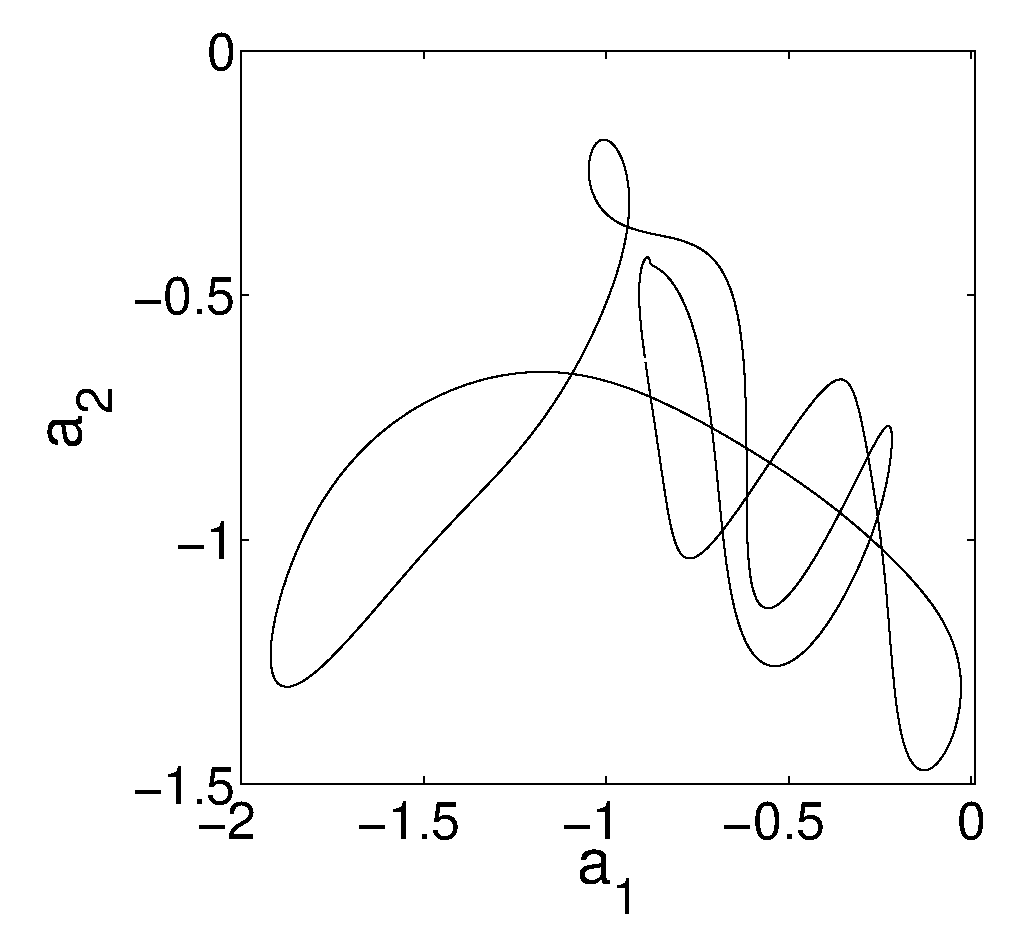
\includegraphics[width=1.8in]{figs/ks21.eps}%
% 	\hspace{0.2cm}%
% 	(b)~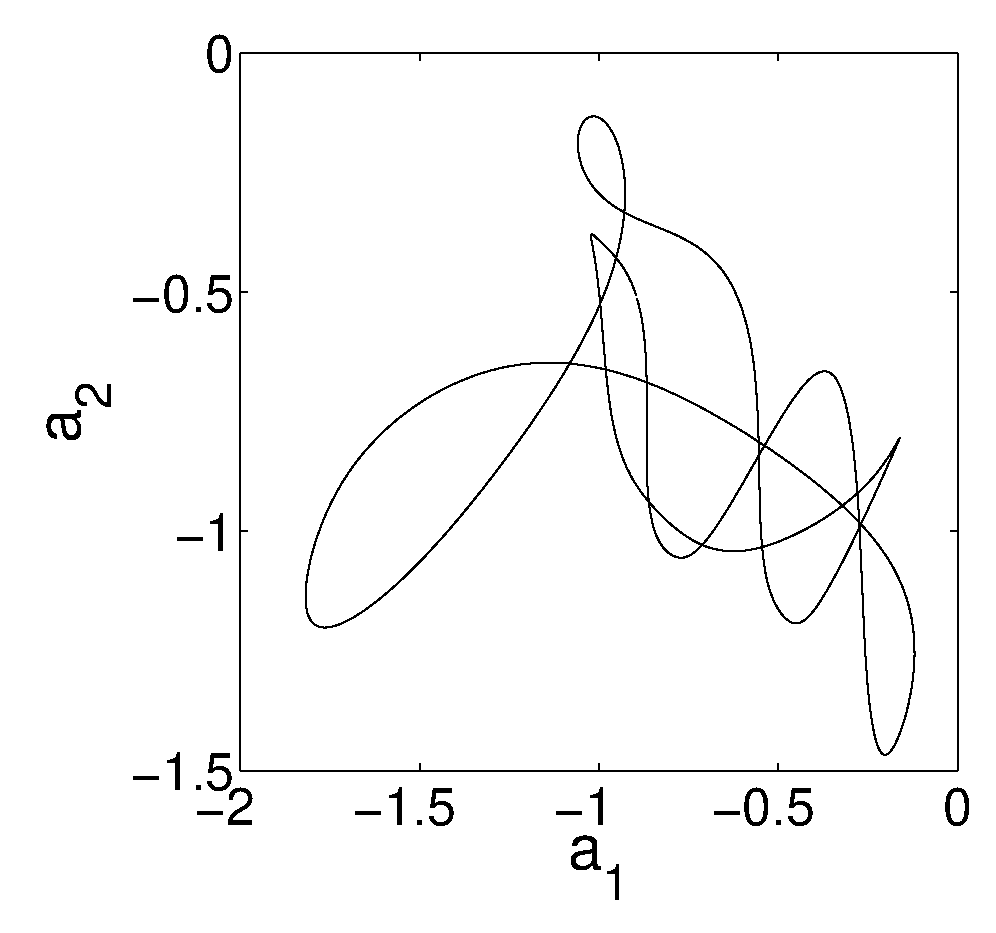
\includegraphics[width=1.8in]{figs/ks22.eps}
% \caption{
%  My System in the
%  chaotic regime (greasy parameter
%  $\nu=0.015$, $d=32$ modes truncation). 
%  (a) An initial guess $L_1$, and 
%  (b) the periodic orbit $p_1$ of period $\period{1}=0.744892$ 
%  determined by My Method.
% 	}
% \label{f:ks1}
% \end{figure}  
%%%%%%%%%%%%%%%%%%%%%%%%%%%%%%%%%%%%%%%%%%%%%%%%%%%%%%%%%%%%%

\section{Discussion}
\label{sec:sum}

The result of this project needs further refinement. The form of \refeq{eq:PDE}
can pose some computational difficulties and a different parameterization or
ansatz needs to be implemented.

Most importantly we still did not incorporate information about the dynamics. Our
suggested solution is to work with the cost functional
\beq
  	F^2 = \int_{s_i}^{s_f} d s\, \frac{v^2}{v.\tilde{v}} \tilde{v}_i g_{ij}\tilde{v}_j\,,
\eeq
with
\beq
	g=\left(\JL \mathbf{P}^{\perp}\right)^T  \left(\JL \mathbf{P}^{\perp}\right)
\eeq

The variational principle that would minimize this functional still needs to be 
formulated. 

%\begin{acknowledgments}

%I would like to thank Mason Porter for 
%numerous helpful suggestions, and
%my mother for bringing \refrefs{HLB96,CCP96} 
%to my attention.

%\end{acknowledgments}         



%%%%%%%%%%%%%%%%%%%%%%%%%%%%%%%%%%%%%%%%%%%%%%%%%%%%%%%%%%%%%

 \bibliographystyle{apsrev}
 \bibliography{refs}
 \nocite{infdymnon,Lan:Thesis,Holmes:96}

\end{document}
